\documentclass[12pt,a4paper]{article}
\usepackage[utf8]{inputenc}
\usepackage[polish]{babel}
\usepackage{polski}
\usepackage{pgfplots}
\usepackage{listings}
\lstset{language=Java}
\usepackage{hyperref}
\usepackage{tikz}
\usetikzlibrary{arrows,shapes}
\pgfplotsset{width=10cm}
\usepackage[left=1cm,right=1cm,top=2cm,bottom=2cm]{geometry}
	\usepackage{fancyhdr}
	\pagestyle{fancy}
	\lhead{Inżynieria oprogramowania} % określa lewą część nagłówka
	\chead{PeerSharing} % określa środkową część nagłówka
	\rhead{Zdzisław Perkowski} % określa prawą część nagłówka
	\lfoot{} % określa lewą część stopki
	\cfoot{\thepage} % określa środkową część stopki
	\rfoot{} % określa prawą część stopki
\author{Zdzisław Perkowski}
\title{PeerSharing}

\begin{document}

\tikzstyle{vertex}=[circle,fill=black!25,minimum size=20pt,inner sep=0pt]
\tikzstyle{selected vertex} = [vertex, fill=red!24]
\tikzstyle{edge} = [draw,thick,-,black!50]
\tikzstyle{weight} = [font=\tiny, color=black]
\tikzstyle{selected edge} = [draw,line width=5pt,-,red!50]
\tikzstyle{ignored edge} = [draw,line width=5pt,-,black!30]

\maketitle
\tableofcontents
\pagebreak


\section{Opis}
Aplikacja \textit{PeerSharing} pozwala na wysyłanie plików między telefonami podłączonymi do tej samej sieci.

\begin{center}
\href{https://github.com/zperkowski/PeerSharing}{GitHub.com/zperkowski/PeerSharing}
\end{center}

\subsection{Pojęcia}
\begin{description}
	\item[Smartphone lub urządzenie] to urządzenie mobilne, które posiada system operacyjny Android w wersji 4.4 lub nowszej. Jednocześnie na tym urządzeniu jest zainstalowany i uruchomiony program oraz urządzenie jest podłączone do sieci.
	\item[Użytkownik] jest to osoba aktualnie obsługująca program za pomocą smartphona.
	\item[Program] to program \textit{PeerSharing}, która aktualnie działa na urządzeniu użytkownika i może wykonywać operacje w tle.
\end{description}

\subsection{Opis programu}

W dalszej części dokumentacji program \textit{PeerSharing} będzie nazywany \textit{programem}.

Program pozwala na wymianę plików między urządzeniami znajdującymi się w tej samej sieci komputerowej. Użytkownik ma możliwość znalezienia innego urządzenia oraz wybrania interesującego go pliku w celu pobrania go na własne urządzenie. Program wysyła pliki za pomocą sieci komputerowej.

\section{Wymagania funkcjonalne}
W tej sekcji znajduje się opis wymagań funkcjonalnych. Wiersz oznaczony gwiazdką (\textbf{*}) oznacza, że jest to czynność opcjonalna, niewpływająca na pozostałe czynności.

\begin{enumerate}
	\item Program pozwala wyszukać inne urządzenia posiadające działający program oraz które są podłączone do tej samej sieci.
	\item Program pozwala przeszukiwać foldery, które zostały udostępnione w programie na innych urządzeniach.
	\item Program pozwala zobaczyć udostępnione dane tylko z jednego urządzenia w danej chwili.
	\item Program wymaga połączenia z siecią do poprawnego działania.
	\item Użytkownik może wybrać maksymalnie jeden plik do pobrania.
\end{enumerate}

\begin{center}
\subsection{Aktualizowanie listy urządzeń bezpośrednio po włączeniu}
	\begin{tabular}{|l|p{5em}|p{30em}|}
	\hline 
	 & Wykonawca & Czynność \\ 
	\hline
	1 & Użytkownik & Włączenie programu. \\
	\hline
	2 & Program & Program prezentuje dostępne urządzenia z zainstalowanym i włączonym programem. \\
	\hline
\end{tabular}
	
\subsection{Pobieranie pliku}
\begin{tabular}{|l|p{5em}|p{30em}|}
	\hline 
	 & Wykonawca & Czynność \\
	\hline 
	1 & Użytkownik & Odświeżenie listy dostępnych urządzeń w sieci. \\ 
	\hline 
	2 & Użytkownik & Wybranie urządzenia z listy dostępnych urządzeń. \\ 
	\hline 
	3* & Użytkownik & Wybranie katalogu w celu wyświetlenia jego zawartości. \\
	\hline
	4 & Użytkownik & Wybranie pliku do pobrania. \\
	\hline
	5 & Program & Pobranie wybranego pliku. \\
	\hline
\end{tabular} 
	
\subsection{Komunikat błędu po włączeniu programu bez połączenia z siecią}
\begin{tabular}{|l|p{5em}|p{30em}|}
	\hline 
	 & Wykonawca & Czynność \\
	\hline
	1 & Użytkownik & Włączenie programu. \\
	\hline
	2 & Program & Próba przeszukania sieci przy braku połączenia z siecią. \\
	\hline
	3 & Program & Wyświetlenie komunikatu o braku połączenia. \\
	\hline
\end{tabular}

\subsection{Komunikat błędu po użyciu wyszukiwania urządzeń bez połączenia z siecią}
\begin{tabular}{|l|p{5em}|p{30em}|}
	\hline 
	 & Wykonawca & Czynność \\
	\hline
	1 & Użytkownik & Chęć zaktualizowania listy dostępnych urządzeń. \\
	\hline
	2 & Program & Próba przeszukania sieci przy braku połączenia z siecią. \\
	\hline
	3 & Program & Wyświetlenie komunikatu o braku połączenia. \\
	\hline
\end{tabular}
\end{center}

\section{Wymagania pozafunkcjonalne}

\begin{itemize}
	\item Program działa na urządzeniach z Androidem w wersji 4.4 Kitkat lub nowszej.
	\item Znalezienie drugiego urządzenia do wymiany plików będzie możliwe po maksymalnie 5 sekundach.
	\item Program będzie przesyłać pliki z szybkośćią na jaką pozwala konfiguracja sieci z którą są urządzenia podłączone.
\end{itemize}
\pagebreak
\section{Makiety}
\subsection{Ekran główny}
Użytkownik ma do wyboru znalezione urządzenia w sieci. Wybranie urządzenia spowoduje zaprezentowanie listy udostępnianych plików przez wybrane urządzenie. Na ekranie jest możliwość zaktualizowania listy dostępnych urządzeń w sieci.
\begin{center}
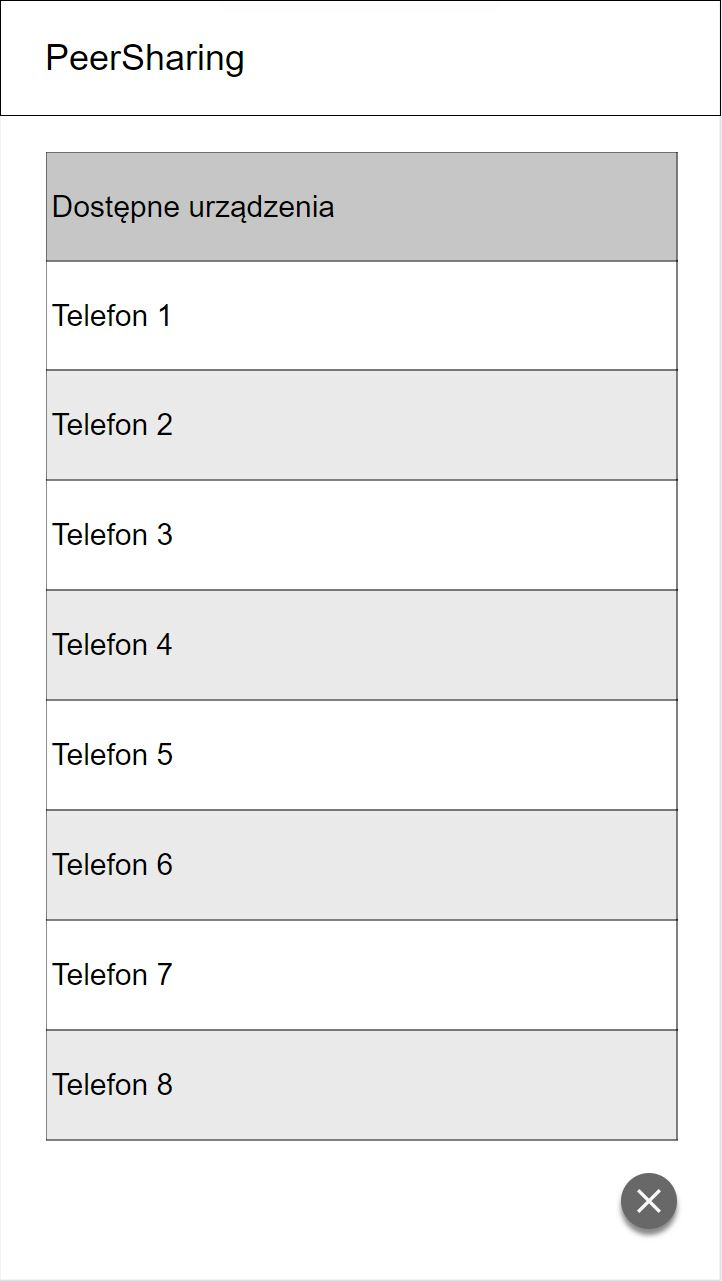
\includegraphics[scale=0.6]{1.JPG}
\end{center}

\subsection{Lista plików}
Po wybraniu urządzenia program prezentuję listę plików i katalogów dostępnych do pobrania. Wybranie katalogu spowoduje prezentacje jego zawartości, wybranie pliku spowoduje jego pobranie.
\begin{center}
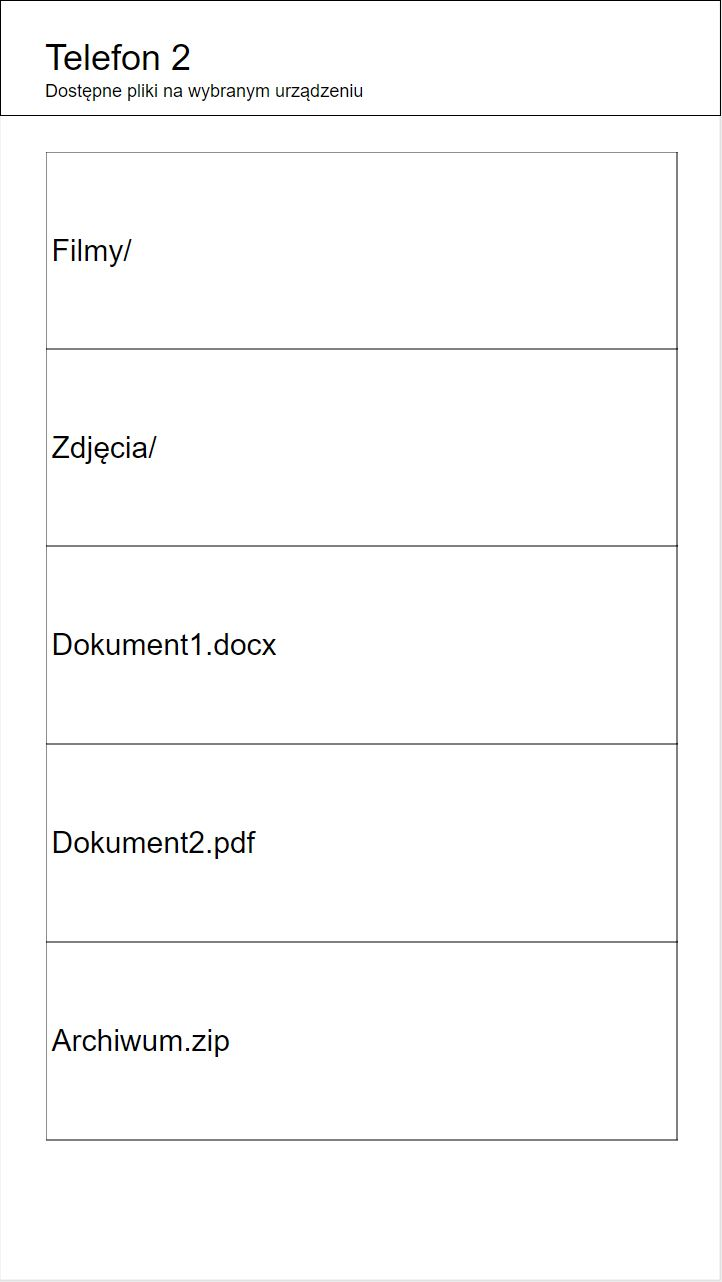
\includegraphics[scale=0.6]{2.JPG}
\end{center}

\end{document}